%!TEX root = ../main.tex
\section{Basic Model under Ambiguity}
\begin{frame}\begin{center}
\LARGE\textbf{Basic Model under Ambiguity}
\end{center}\end{frame}
%------------------------------------------------------------------------------- 
%------------------------------------------------------------------------------- 
\begin{frame}
\begin{itemize}\setlength\itemsep{1em}
\item Modeling Ambiguity\medskip
\item Understanding Economic Mechanism\medskip
\item Assessing Model Misspecification\medskip
\end{itemize}
\end{frame}
%-------------------------------------------------------------------------------
%-------------------------------------------------------------------------------
\subsection{Modeling Ambiguity}
\begin{frame}\begin{center}
\LARGE\textit{Modeling Ambiguity}
\end{center}\end{frame}


\begin{frame}
To fix ideas, let us study the decision problem of \textit{Agent Blue} in the second to last period:

\begin{itemize}\setlength\itemsep{1em}
\item 9 Years of Experience in Occupation A
\item 20 Years of  Experience in Occupation B
\item 1 Year of Additional Schooling
\end{itemize}
\end{frame}
%-------------------------------------------------------------------------------
%-------------------------------------------------------------------------------
\begin{frame}
\textbf{Set of Admissible Beliefs}\medskip
\begin{align*}
\N = \{\mathcal{N} \in \mathrm{Q}: D_{KL}(\mathcal{N}_0\mid \mathcal{N}) \leq \theta\}
\end{align*}


\textit{Distribution of Labor Market Shocks}

\scriptsize\begin{eqnarray*}
\begin{pmatrix}
\epsilon_{1,t}\\
\epsilon_{2,t}
\end{pmatrix} & \sim & \mathcal{N}\left[\left(\begin{array}{c}
\mu_{\epsilon_{1, t}}\\
\mu_{\epsilon_{2, t}}
\end{array}\right),\left(\begin{array}{cccc}
16\times10^{-4}  &   0.00   \\
0.00            &   25\times10^{-2}
\end{array}\right)\right]
\end{eqnarray*}



\end{frame}
%-------------------------------------------------------------------------------
%-------------------------------------------------------------------------------
\begin{frame}
\begin{center}\textbf{Exploring Set of Admissible Beliefs}
\scalebox{0.38}{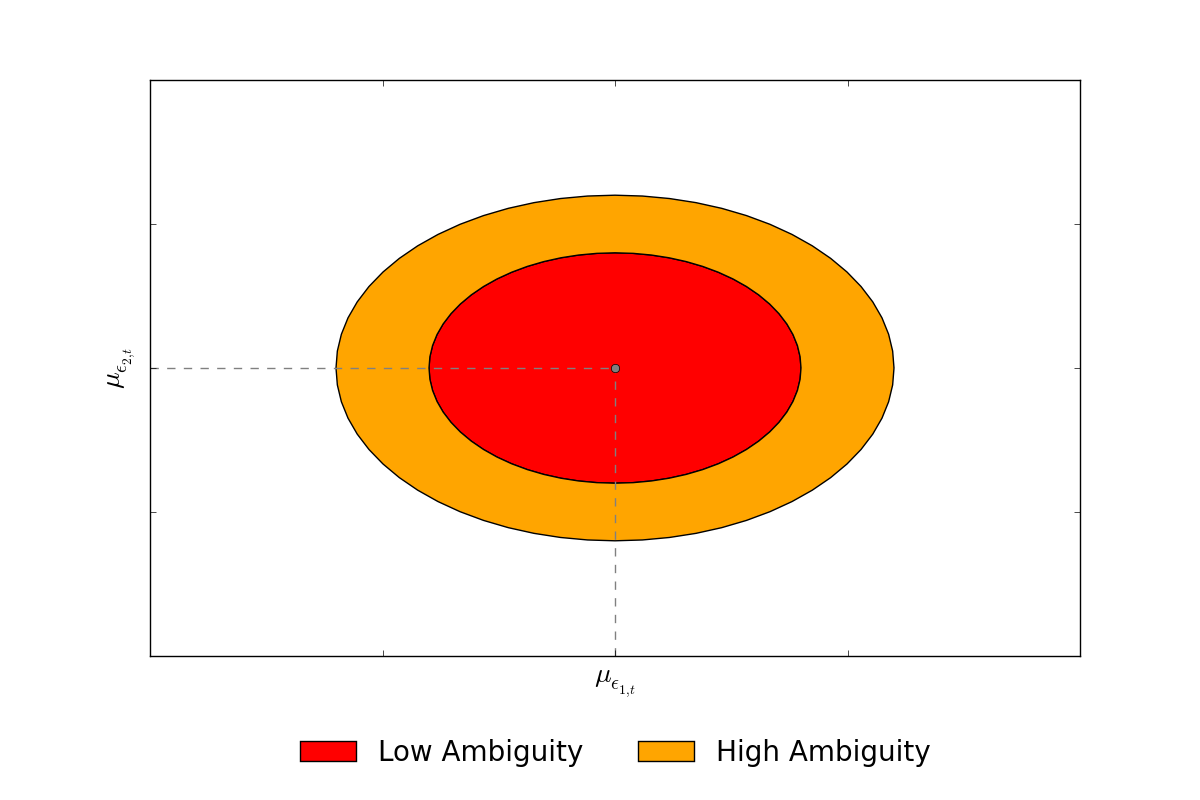
\includegraphics{../material/exploring_entropy}}
\end{center}
\end{frame}
%-------------------------------------------------------------------------------
%-------------------------------------------------------------------------------
\begin{frame}
\begin{center}\textbf{Exploring Admissible Value Functions}\vspace{0.3cm}
\scalebox{0.38}{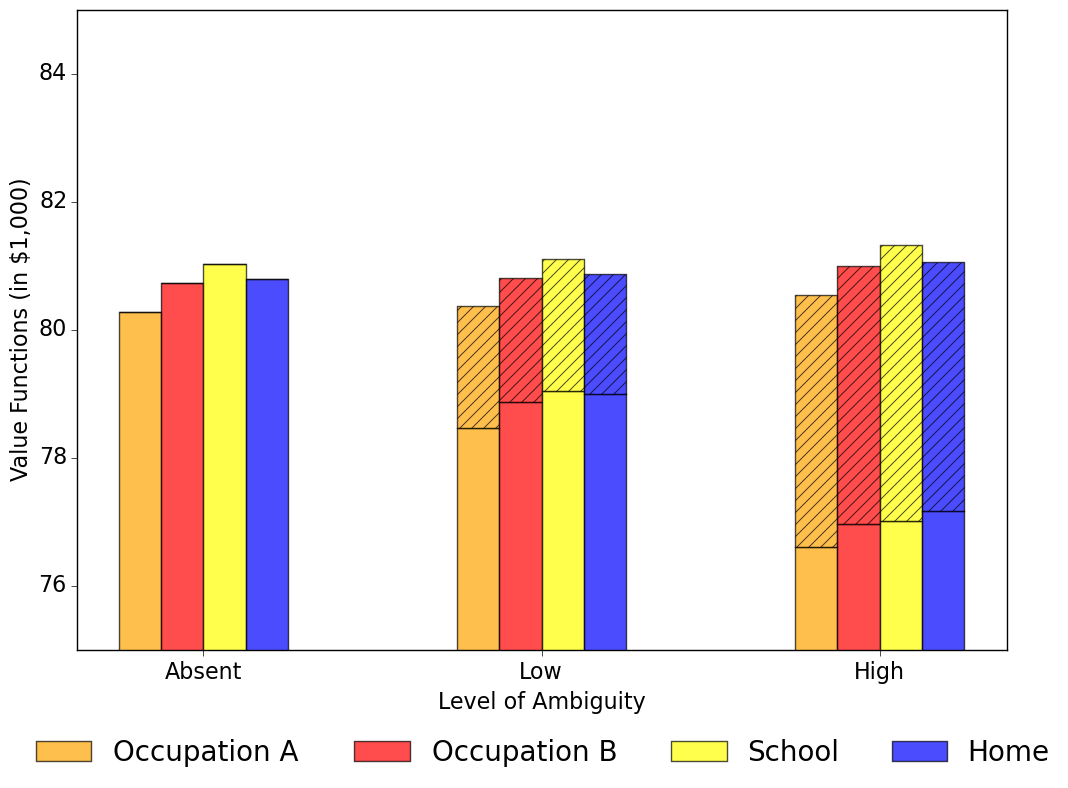
\includegraphics{../material/admissible_values}}
\end{center}
\end{frame}
%-------------------------------------------------------------------------------
%-------------------------------------------------------------------------------
\begin{frame}\vspace{0.75cm}
\textbf{Agents' Objective under Ambiguity}\vspace{0.3cm}
\begin{align*} 
V^*(S(t),t) = \max_{\{d_k(t)\}_{k \in K}} \left\{ \min_{\pmb{\mathcal{N}} \in \pmb{\mathbb{N}}}E_{\pmb{\mathcal{N}}}\left[ \sum_{\tau = t}^T \delta^{\tau - t} \sum_{k\in K}R_k(\tau)d_k(\tau)\Bigg| S(t)\right]\right\}\\
\end{align*}

\vspace{0.5cm}
\textbf{See:} \citet{Epstein.2003}, \citet{Hansen.2007}
\end{frame}
%-------------------------------------------------------------------------------
%-------------------------------------------------------------------------------
\begin{frame}
\textbf{Bellman Equations}\vspace{0.3cm}
\begin{align*}\small
V^*(S(t),t) = \max_{k \in K}\{V^*_k(S(t),t)\},
\end{align*}
where for all but the final period:
\begin{align*}
V^*_k(S(t),t) = R_k(S(t),t) + \delta \min_{\mathcal{N} \in \mathbb{N}}E_\mathcal{N}\left[V^*(S(t + 1), t + 1)\mid\cdot\thin\right] \end{align*}

\vspace{0.5cm}
\textbf{See:} \citet{Iyengar.2005}

\end{frame}
%-------------------------------------------------------------------------------
%-------------------------------------------------------------------------------
\subsection{Understanding Economic Mechanism}
\begin{frame}\begin{center}
\LARGE\textit{Understanding Economic Mechanism}
\end{center}\end{frame}
%-------------------------------------------------------------------------------
%-------------------------------------------------------------------------------
\begin{frame}
\textbf{Quantifying Level of Ambiguity}\vspace{0.3cm}
\begin{center}
  \begin{tabular}{C{1.8cm}  C{2.5cm} C{3.0cm} C{1.5cm}}\toprule
     Ambiguity  & Lifetime Value   & Relative Change & $\theta$\\\toprule
    Absent  & \$405,258    & --- & 0.0000\\
    Low     & \$395,129   & -2.5\%& 0.0033\\
    High    & \$384,988    & -5.0\%& 0.0142\\\bottomrule
  \end{tabular}
\end{center}
\end{frame}
%-------------------------------------------------------------------------------
%-------------------------------------------------------------------------------
\begin{frame}
\begin{center}\textbf{Changing Schooling Investment}\vspace{0.3cm}
    \scalebox{0.38}{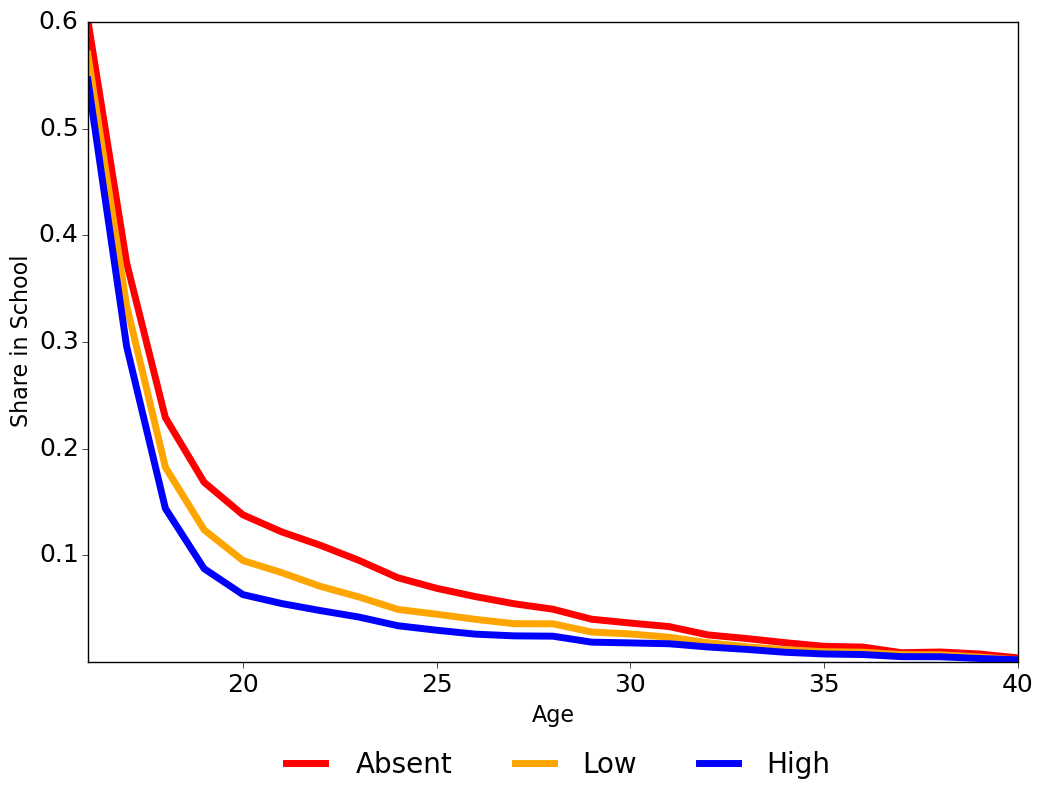
\includegraphics{../material/schooling_ambiguity}}
\end{center}
\end{frame}
%-------------------------------------------------------------------------------
%-------------------------------------------------------------------------------
\begin{frame}
\textbf{Changing Occupational Sorting}\vspace{0.3cm}


\begin{center}
\begin{tabular}{C{1.8cm} C{2cm} C{2cm} }\toprule
                        & \mc{2}{c}{\underline{Share in Occupation}} \\[-2ex]
     Ambiguity          & A & B  \\\midrule
    Absent & 55\% & 39\%  \\
    Low    & 57\% & 35\%   \\
    High   & 60\% & 32\%   \\\bottomrule
\end{tabular}
\end{center}
\end{frame}
%-------------------------------------------------------------------------------
%-------------------------------------------------------------------------------
\subsection{Assessing Model Misspecification}
\begin{frame}\begin{center}
\LARGE\textit{Assessing Model Misspecification}
\end{center}\end{frame}
%-------------------------------------------------------------------------------
%-------------------------------------------------------------------------------
\begin{frame}
\begin{center}\textbf{Ambiguity and Psychic Costs}
\begin{figure}[h!]\centering
\subfloat[Absent]{
\scalebox{0.15}{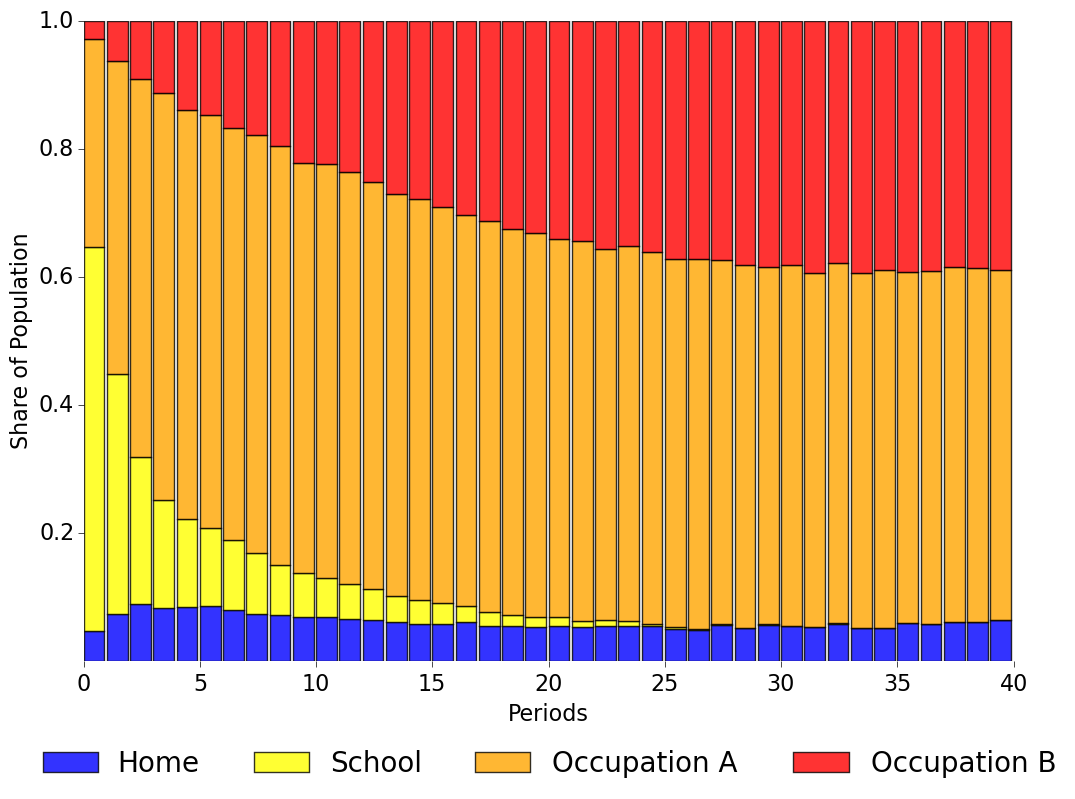
\includegraphics{../material/choice_patterns_0000}}}\\\vspace{-0.3cm}
\subfloat[Low]{\
\scalebox{0.15}{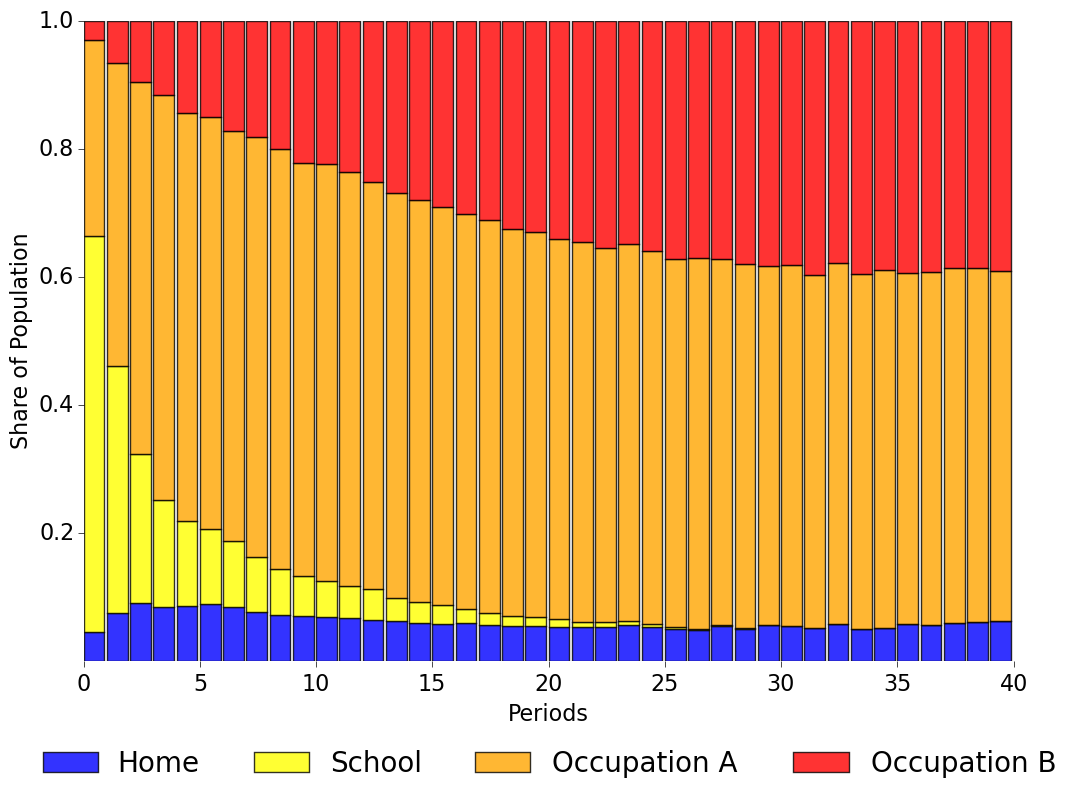
\includegraphics{../material/choice_patterns_0033}}}\hspace{1.0cm}
\subfloat[High]{\
\scalebox{0.15}{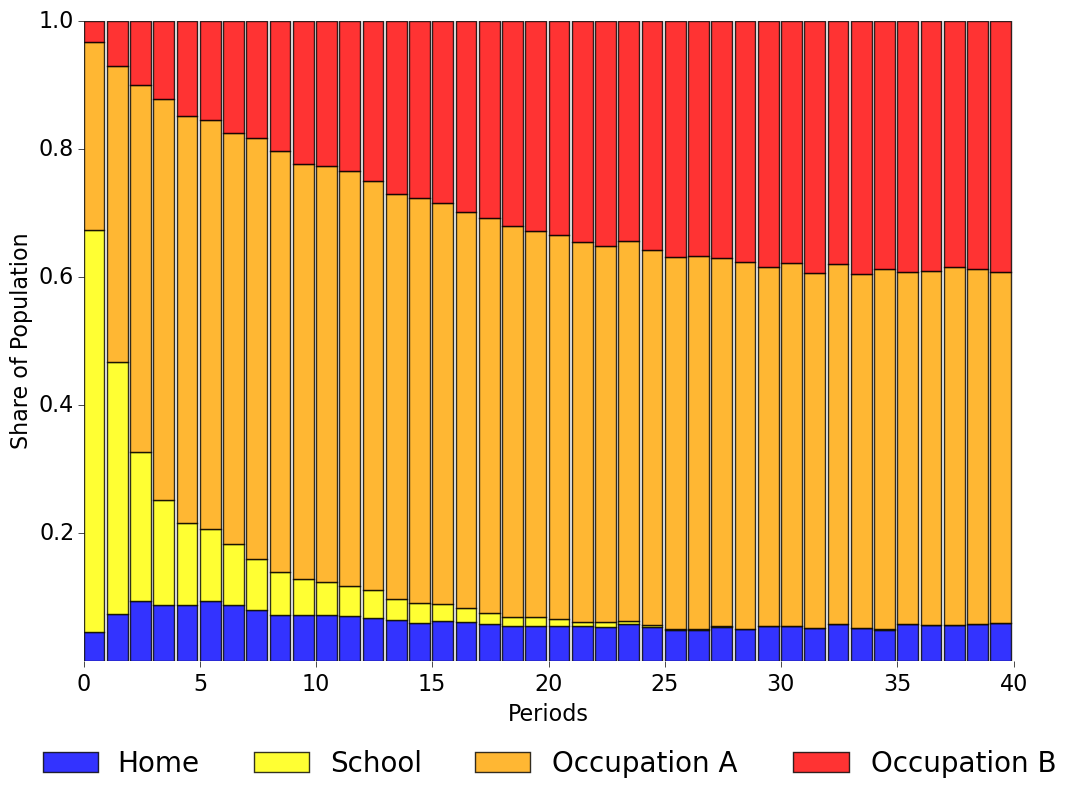
\includegraphics{../material/choice_patterns_0142}}}
\end{figure}\end{center}\end{frame}
%-------------------------------------------------------------------------------
%-------------------------------------------------------------------------------
\begin{frame}
\begin{center}\textbf{Modeling Trade-off}\vspace{0.3cm}
\scalebox{0.38}{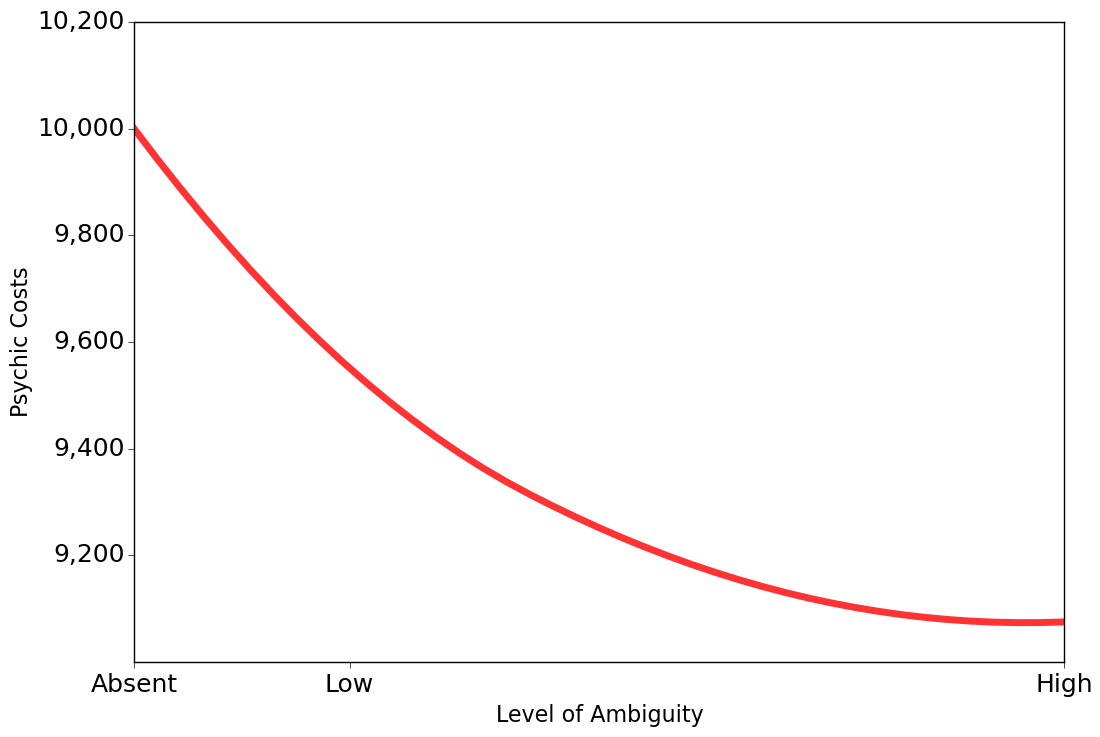
\includegraphics{../material/indifference_curve}}
\end{center}
\end{frame}

%-------------------------------------------------------------------------------
%-------------------------------------------------------------------------------
\begin{frame}\textbf{Model Misspecification and Psychic Costs Estimates}\vspace{0.3cm}


\begin{center}
\begin{tabular}{C{1.8cm} C{2cm} C{2cm}  C{2cm}}\toprule
                        & \mc{3}{c}{\underline{Psychic Costs}}  \\[-2ex]
     Ambiguity          & True & Estimate  & Discrepancy\\\midrule
    Absent & 10,000 & 10,000  & ---\\
    Low    &  9,550 & 10,000  &  450  \\
    High   &  9,075 & 10,000  &  925\\\bottomrule
\end{tabular}
\end{center}

\end{frame}
%-------------------------------------------------------------------------------
%-------------------------------------------------------------------------------
\begin{frame}\textbf{Model Misspecification and Policy Assessment}\vspace{0.3cm}


\begin{center}
\begin{tabular}{C{1.8cm} C{2cm} C{2cm} C{2cm}}\toprule
                        & \mc{3}{c}{\underline{Average Schooling}}  \\[-2ex]
     Ambiguity          &  True & Estimate & Discrepancy \\\midrule
    Absent & 1.18 & 1.18 & ---\\
    Low    & 1.12 & 1.18 &  0.06\\
    High   & 1.10 & 1.18 & 0.08 \\\bottomrule
\end{tabular}
\end{center}


\end{frame}